\documentclass[12pt]{article}
\usepackage[english]{babel}
\usepackage{url}
\usepackage[utf8x]{inputenc}
\usepackage{amsmath}
\usepackage{graphicx}
\graphicspath{{images/}}
\usepackage{parskip}
\usepackage{fancyhdr}
\usepackage{epsfig}
\usepackage{listings}
\include{import}
\usepackage[T1]{fontenc}
\usepackage{amsmath}
\usepackage{titlesec}
\usepackage{amssymb}
\lstset{basicstyle = \ttfamily}
\usepackage{vmargin}
\usepackage{float}
\usepackage{pdfpages,caption,geometry}
\usepackage[hidelinks]{hyperref}
\setmarginsrb{3 cm}{2.5 cm}{3 cm}{2.5 cm}{1 cm}{1.5 cm}{1 cm}{1.5 cm}
%\setcounter{secnumdepth}{0}         % Removes Section Numbering
\title{VLSI Lab Report}								% Title
\author{\begin{tabular}[t]{l l} 
		Anirudh BH  & 16EC105 \\
		Manan Sharma & 16EC118\\ 
\end{tabular}}								% Author
\date{\today}											% Date
\hypersetup{
	bookmarks=true,         
	unicode=true,         
	pdftoolbar=false,        
	pdfmenubar=false,        
	%pdffitwindow=false,     
	pdfstartview={FitH},    
	pdftitle={VLSI Lab Report}, 
	pdfauthor={Anirudh BH, Manan Sharma},
	pdfsubject={VLSI Lab},
	pdfnewwindow=true,      
}
\titlespacing*{\section}{0pt}{1ex}{1ex}
\titlespacing*{\subsection}{0pt}{0.5ex}{0.5ex}
\titlespacing*{\subsubsection}{0pt}{0.5ex}{0.5ex}
\makeatletter
\let\thetitle\@title
\let\theauthor\@author
\let\thedate\@date
\makeatother

\pagestyle{fancy}
\fancyhf{}
\rhead{Anirudh BH, Manan Sharma}
\lhead{VLSI Lab Report}
\cfoot{\thepage}

\begin{document}
	\begin{titlepage}
		\centering
		\vspace*{0.4 cm}
		
\includegraphics[width = 0.3\textwidth]{NITK_Logo.png}\\[1.0 cm]	% University Logo
		\textsc{\Large National Institute of Technology Karnataka, Surathkal}\\[1.5 cm]	% University Name
		\textsc{\Large EC372}\\[0.5 cm]				% Course Code
		\textsc{\Large VLSI Design Lab}\\[0.5 cm]				% Course Name
		\rule{\linewidth}{0.2 mm} \\[0.4 cm]
		\textbf{\textsc{ \huge  \thetitle}}\\
		\rule{\linewidth}{0.2 mm} \\[1.5 cm]
		\begin{flushleft} \large
			\hspace{0.45em}\emph{Authors:}\\
			\theauthor\\[2 cm]
		\end{flushleft}
		
		{\large \thedate}
		
		\vfill
	\end{titlepage}

	\tableofcontents
	\pagebreak
	
	\section{Study of MOS Inverter with Resistive Load}
	
	\subsection{Objective}
	To study the:
	\begin{enumerate}
		\item Transfer Function
		\item Noise Margin
		\item Risetime and Fall time
		\item Propagation Delay
		\item Power and Energy consumed
	\end{enumerate}
	with variation in $\text{R}_\text{L}$ and W of the load resistor and pull-down transistor. Along with this, also calculate power and energy consumed for non ideal step input for resistive load inverter.
	\subsection{Introduction}
	Inverter is one that inverts the signal supplied at its input. If input is made high or logic level is 1, then the output has logic level 0 and vice-versa. A resistive load inverter is characterised by an resistive load between the pull down transistor and the voltage source. The output is taken at the junction of the load resistance and the pull down transistor. The pull-up circuit is constituted by the resistor and pull-down resistor by the NMOS. When the input is low, the NMOS is open circuited and the output capacitance is charged to $\text{V}_\text{DD}$ through $\text{R}_\text{L}$.
	
	\subsection{Circuit Diagram}
	\begin{figure}[H]
		\begin{center}
			% XCircuit output "resistive_load.tex" for LaTeX input from resistive_load.eps
\def\putbox#1#2#3#4{\makebox[0in][l]{\makebox[#1][l]{}\raisebox{\baselineskip}[0in][0in]{\raisebox{#2}[0in][0in]{\scalebox{#3}{#4}}}}}
\def\rightbox#1{\makebox[0in][r]{#1}}
\def\centbox#1{\makebox[0in]{#1}}
\def\topbox#1{\raisebox{-0.60\baselineskip}[0in][0in]{#1}}
\def\midbox#1{\raisebox{-0.20\baselineskip}[0in][0in]{#1}}
   \scalebox{0.825}{
   \normalsize
   \parbox{1.5625in}{
   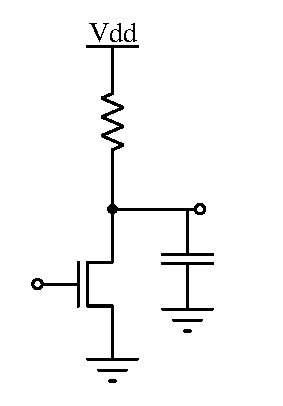
\includegraphics[scale=1]{resistive_load}\\
   % translate x=400 y=316 scale 0.38
   \putbox{0.31in}{1.70in}{1.20}{$\text{R}_\text{L}$}%
   \putbox{1.31in}{1.20in}{1.20}{out}%
   \putbox{0.06in}{0.79in}{1.20}{in}%
   \putbox{1.39in}{0.79in}{1.20}{$\text{C}_\text{L}$}%
   } % close 'parbox'
   } % close 'scalebox'
   \vspace{-\baselineskip} % this is not necessary, but looks better

			\caption{Circuit Diagram of Resistive Load Inverter}
			\label{fig::resloadckt}
		\end{center}
	\end{figure}

	\subsection{Netlist}
    \begin{lstlisting}
    * transistor and other circuit components definition
    m0 out in 0 0 cmosn l=2.5u w=10u
    rl supply out 7k
    cl out meas 5n
    
    * voltage source
    vdd supply 0 dc 3.3
    vin in 0 dc 3.3 pulse(0 3.3 0 0.1n 0.1n 0.5m 1m)
    vcap meas 0 dc 0
    \end{lstlisting}
    
    \subsection{Analysis and Observations}
    
    Transfer characteristics were plotted for different values of $\text{R}_\text{L}$ and different W and L values for the driver NMOS. The plots obtained were as follows:
    
    The curves moving to the right imply that the threshold voltage is increasing and moving to the right. Figure(\ref{fig::varying_rl_dc}) indicates that as $\text{R}_\text{L}$ increases the voltage drop across it increases. This implies that the graph moves to the left as $\text{R}_\text{L}$ increases.\\
    Figure(\ref{fig::varying_rl_time}) indicates that as $\text{R}_\text{L}$ increases the pull up resistance to the load increases. This results in the rise time increasing for an increase in $\text{R}_\text{L}$.\\
    Figure(\ref{fig::varying_rl_vcap}) indicates that as $\text{R}_\text{L}$. increases the peak current drawn by the capacitor decreases. Figure(\ref{fig::varying_rl_vdd}) indicates that the current drawn from $\text{V}_{\text{DD}}$ is the same.
    \begin{figure}[H]
		\begin{center}
			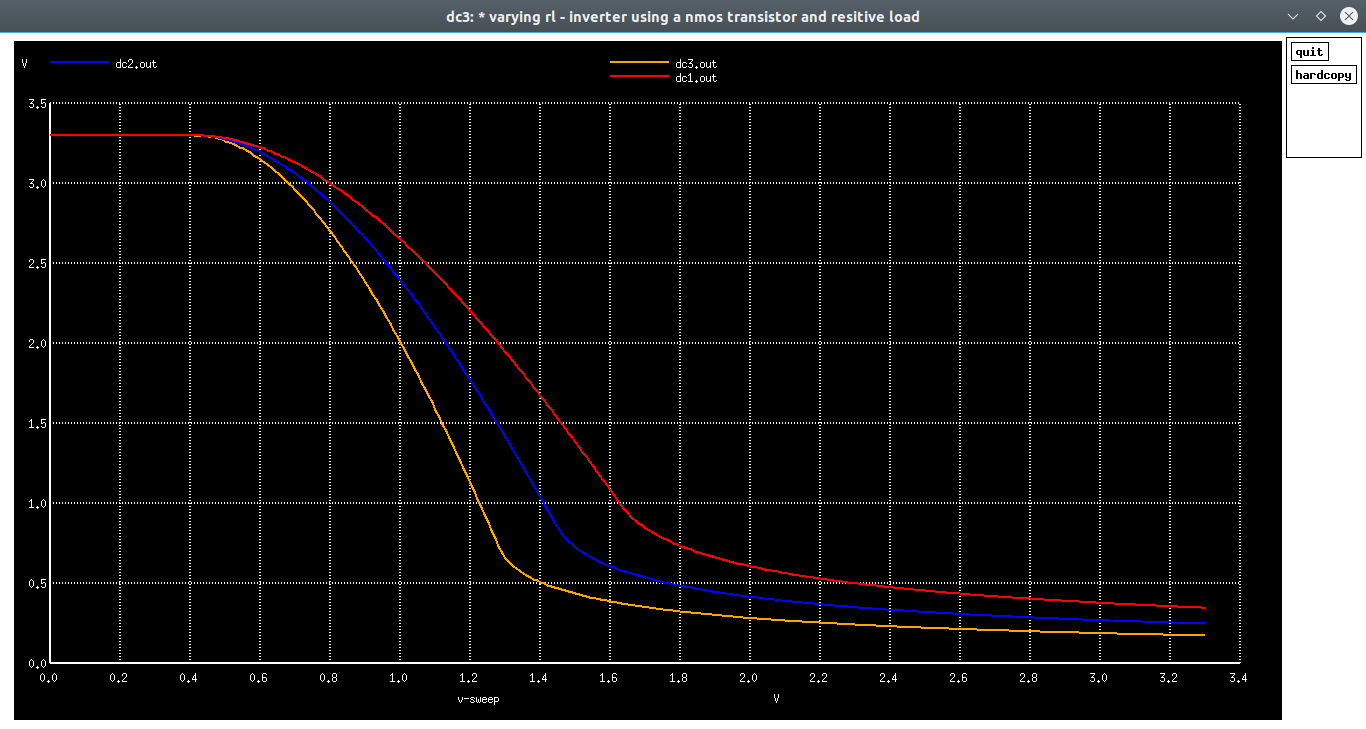
\includegraphics[scale=0.25]{images/inverter_Rl_dc.png}
			\caption{Transfer Characteristics Varying $\text{R}_\text{L}$(left to right: 10K, 7K, 5K)}
			\label{fig::varying_rl_dc}
		\end{center}
	\end{figure}
	\begin{figure}[H]
		\begin{center}
			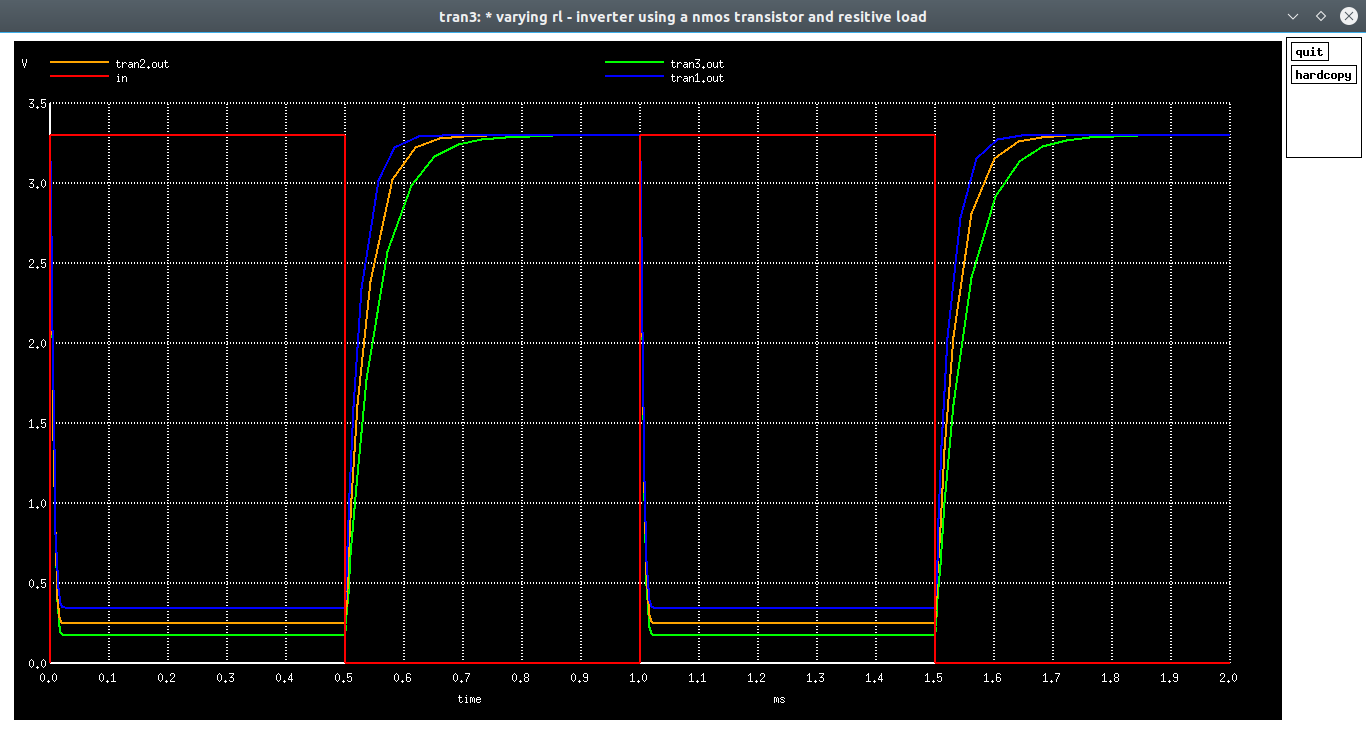
\includegraphics[scale=0.25]{images/inverter_Rl_tran.png}
			\caption{Transient Response Varying $\text{R}_\text{L}$(left to right: 5K, 7K, 10K)}
			\label{fig::varying_rl_time}
		\end{center}
	\end{figure}
	
	\begin{figure}[H]
		\begin{center}
			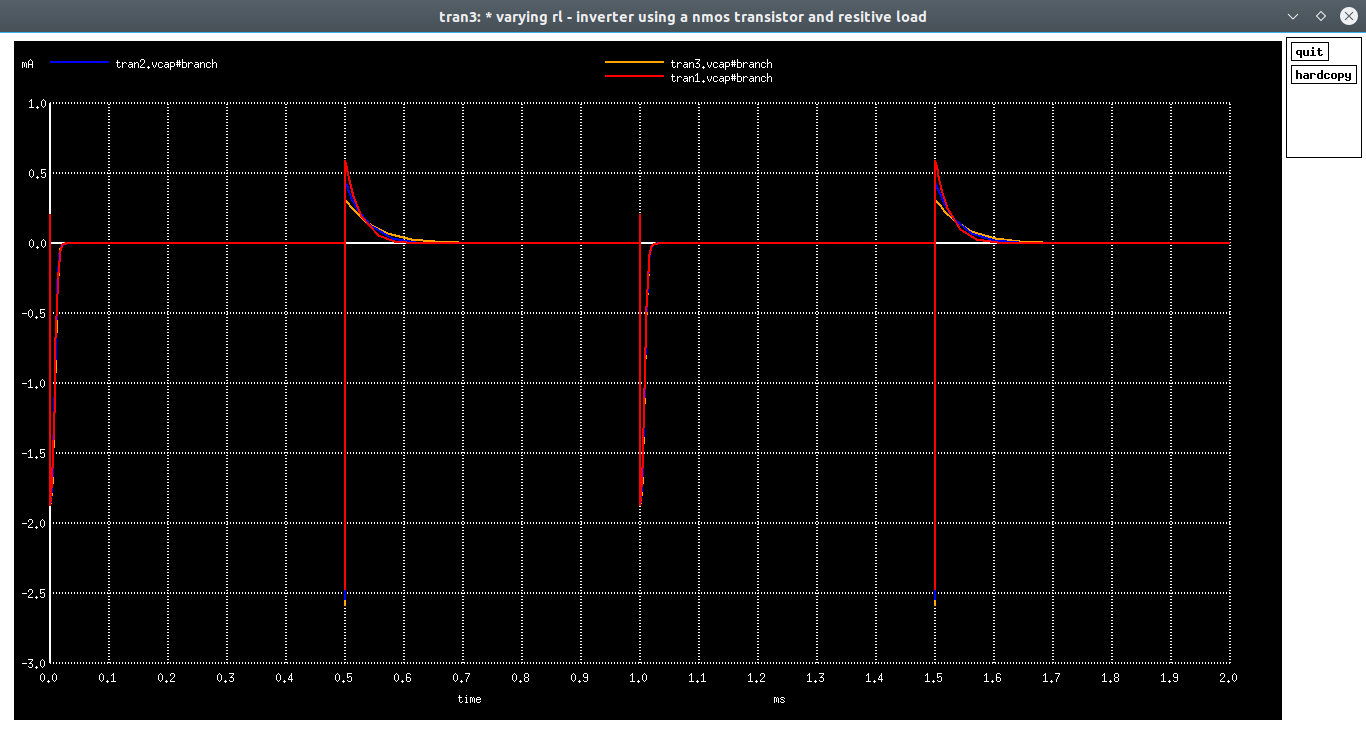
\includegraphics[scale=0.25]{images/inverter_Rl_vcap.png}
			\caption{Capacitor Current Varying $\text{R}_\text{L}$}
			\label{fig::varying_rl_vcap}
		\end{center}
	\end{figure}
	
	\begin{figure}[H]
		\begin{center}
			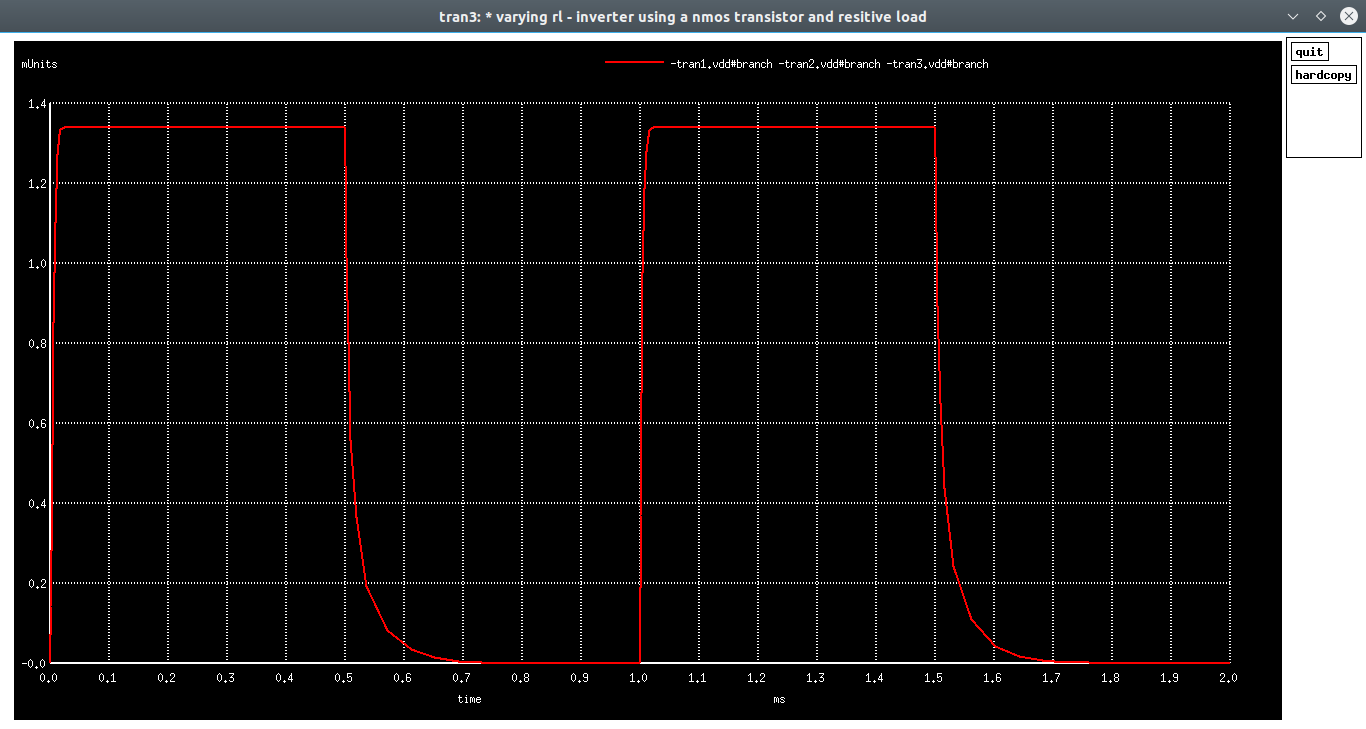
\includegraphics[scale=0.25]{images/inverter_Rl_vdd.png}
			\caption{Transient Response Varying $\text{R}_\text{L}$}
			\label{fig::varying_rl_vdd}
		\end{center}
	\end{figure}
	
	Figure(\ref{fig::varying_w_dc}) indicates that as W increases the voltage drop across the load $\text{R}_\text{L}$ increases. This implies that the graph moves to the left as W increases.\\
    Figure(\ref{fig::varying_w_time}) indicates that as W increases the pull-down resistance to the ground decreases. This results in the rise time decreaseing for an increase in W.\\
    Figure(\ref{fig::varying_w_vcap}) indicates that as W increases the peak current drawn by the capacitor increases. Figure(\ref{fig::varying_w_vdd}) indicates that the current drawn from $\text{V}_{\text{DD}}$ is the same.
    \begin{figure}[H]
		\begin{center}
			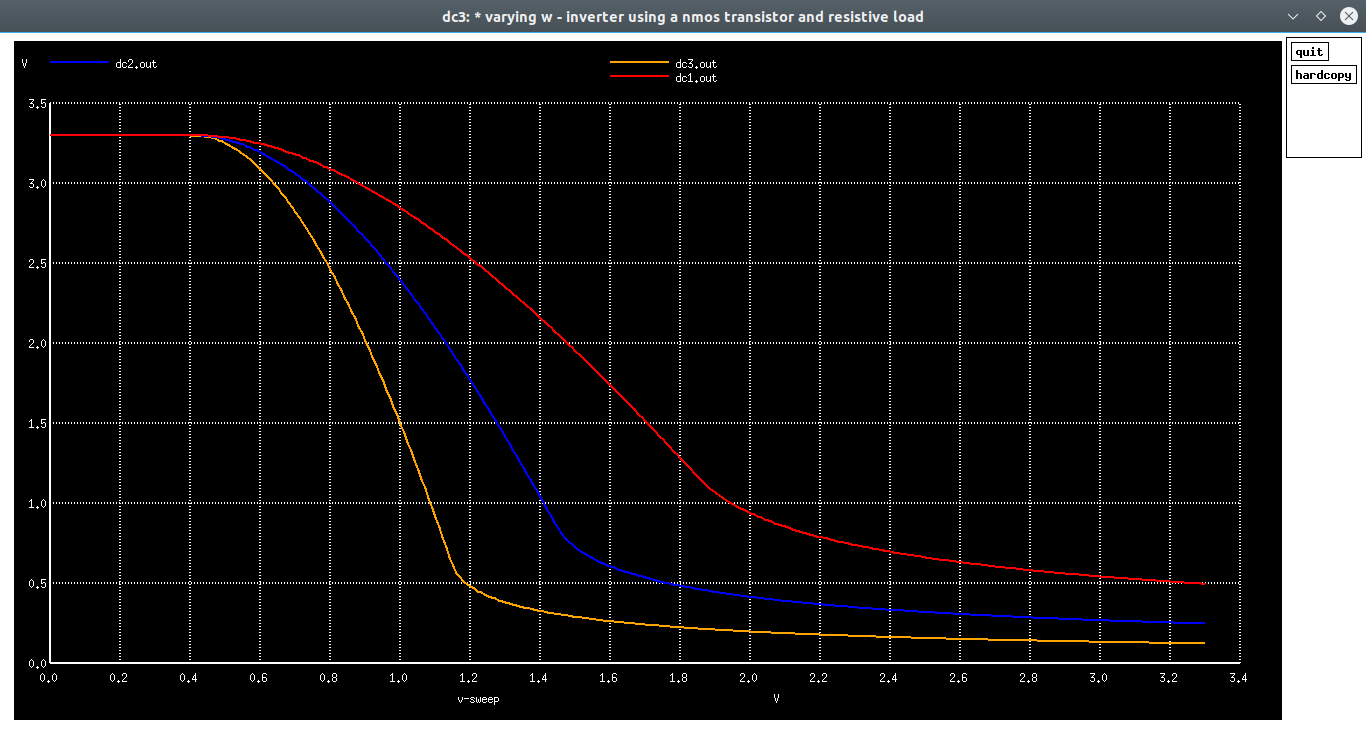
\includegraphics[scale=0.25]{images/inverter_w_dc.png}
			\caption{Transfer Characteristics Varying W}
			\label{fig::varying_w_dc}
		\end{center}
	\end{figure}
	\begin{figure}[H]
		\begin{center}
			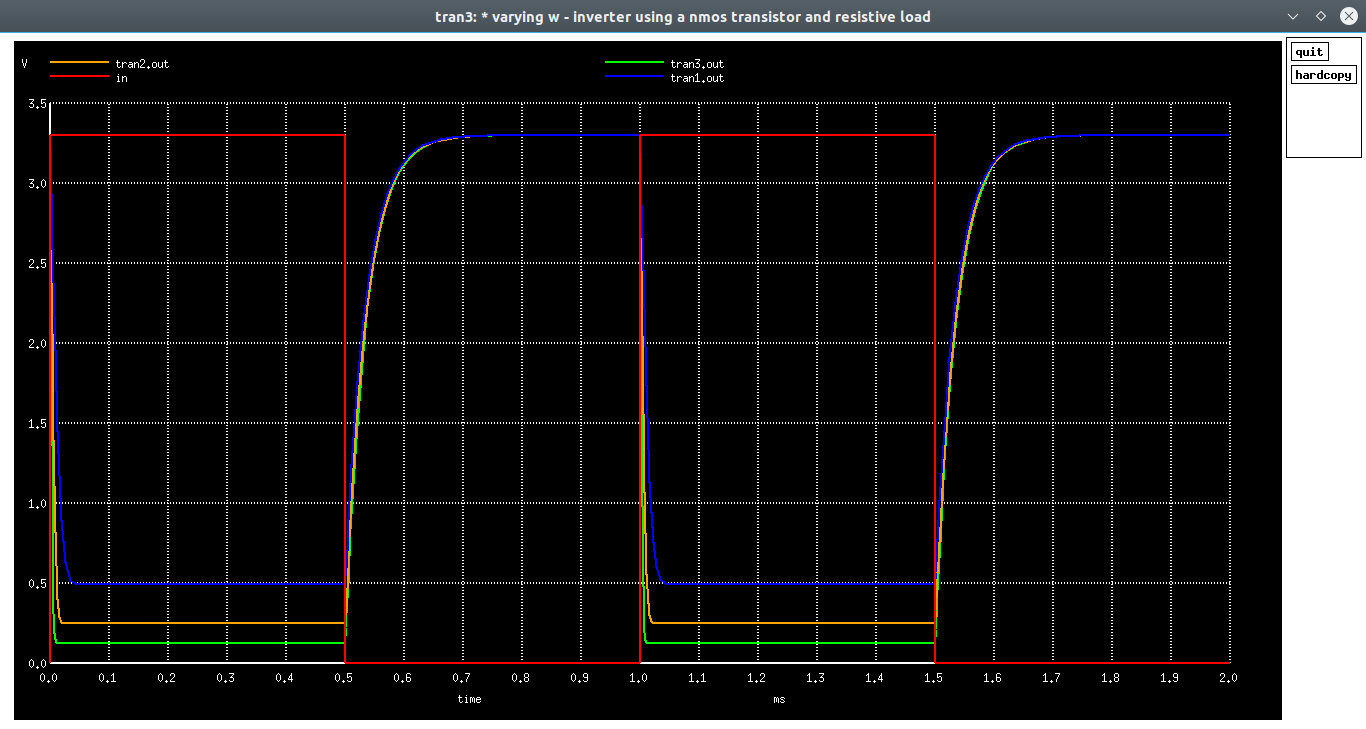
\includegraphics[scale=0.25]{images/inverter_w_tran.png}
			\caption{Transient Response Varying W}
			\label{fig::varying_w_time}
		\end{center}
	\end{figure}
	
	\begin{figure}[H]
		\begin{center}
			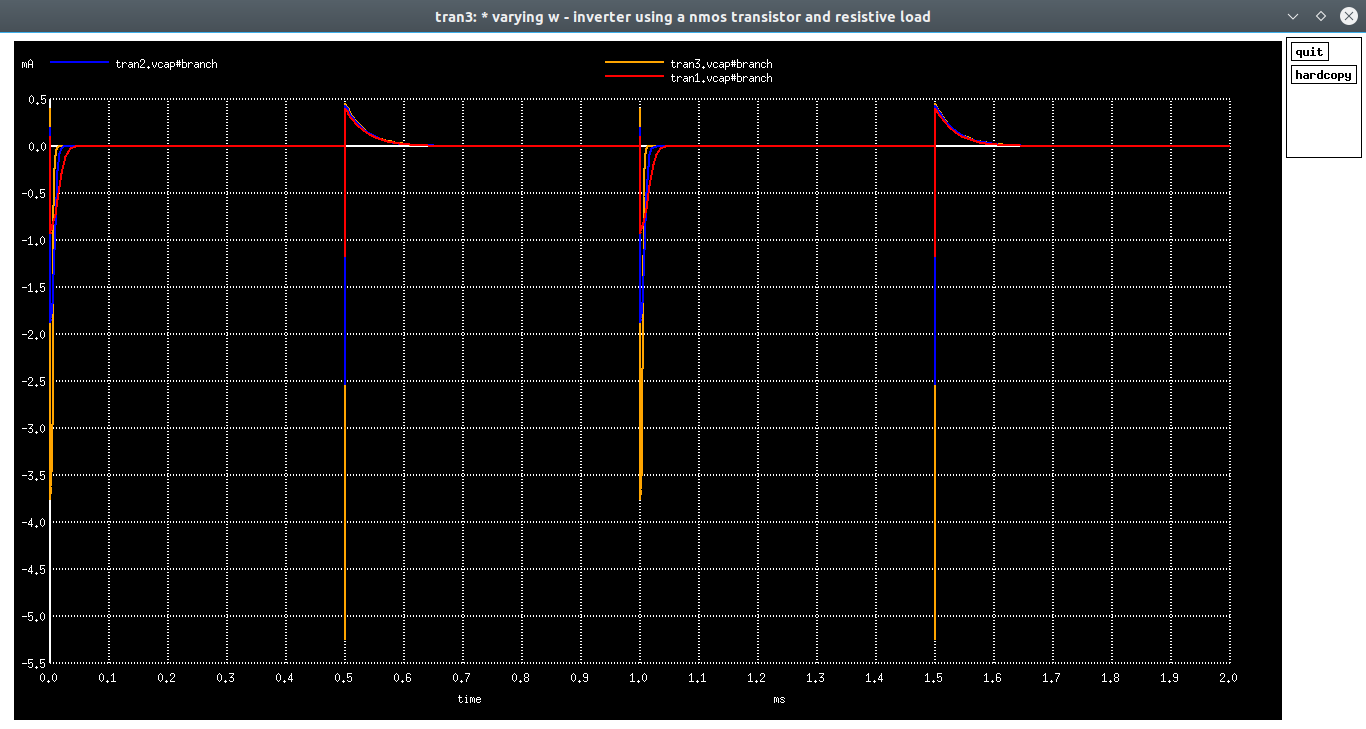
\includegraphics[scale=0.25]{images/inverter_w_vcap.png}
			\caption{Capacitor Current Varying W}
			\label{fig::varying_w_vcap}
		\end{center}
	\end{figure}
	
	\begin{figure}[H]
		\begin{center}
			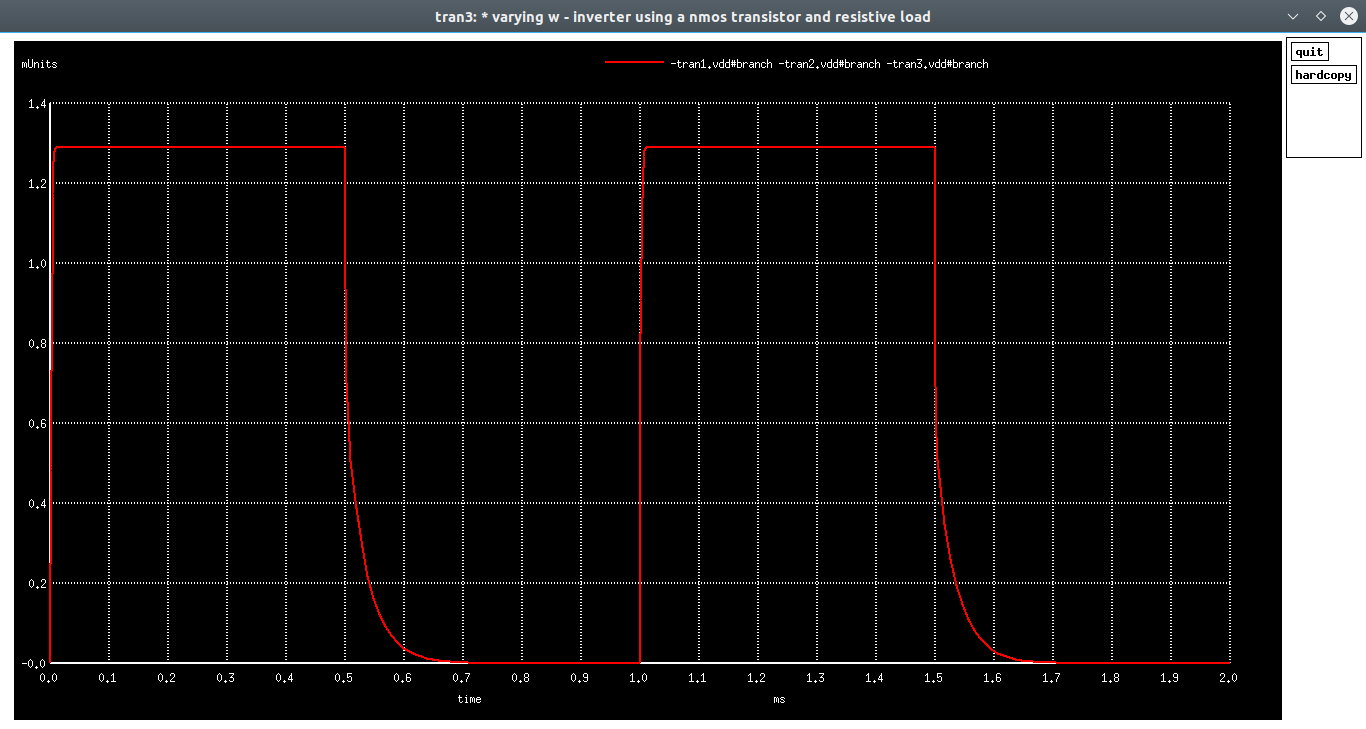
\includegraphics[scale=0.25]{images/inverter_w_vdd.png}
			\caption{Transient Response Varying W}
			\label{fig::varying_w_vdd}
		\end{center}
	\end{figure}
	
	
	Figure(\ref{fig::varying_l_dc}) indicates that as L increases, the current decreases and the voltage drop across the load $\text{R}_\text{L}$ decreases. This implies that the graph moves to the right as L increases.\\
    Figure(\ref{fig::varying_l_time}) indicates that as L increases the pull-down resistance to the ground increases. This results in the rise time increasing for an increase in L.\\
    Figure(\ref{fig::varying_l_vdd}) indicates that the current drawn from $\text{V}_{\text{DD}}$ is the same.
    \begin{figure}[H]
		\begin{center}
			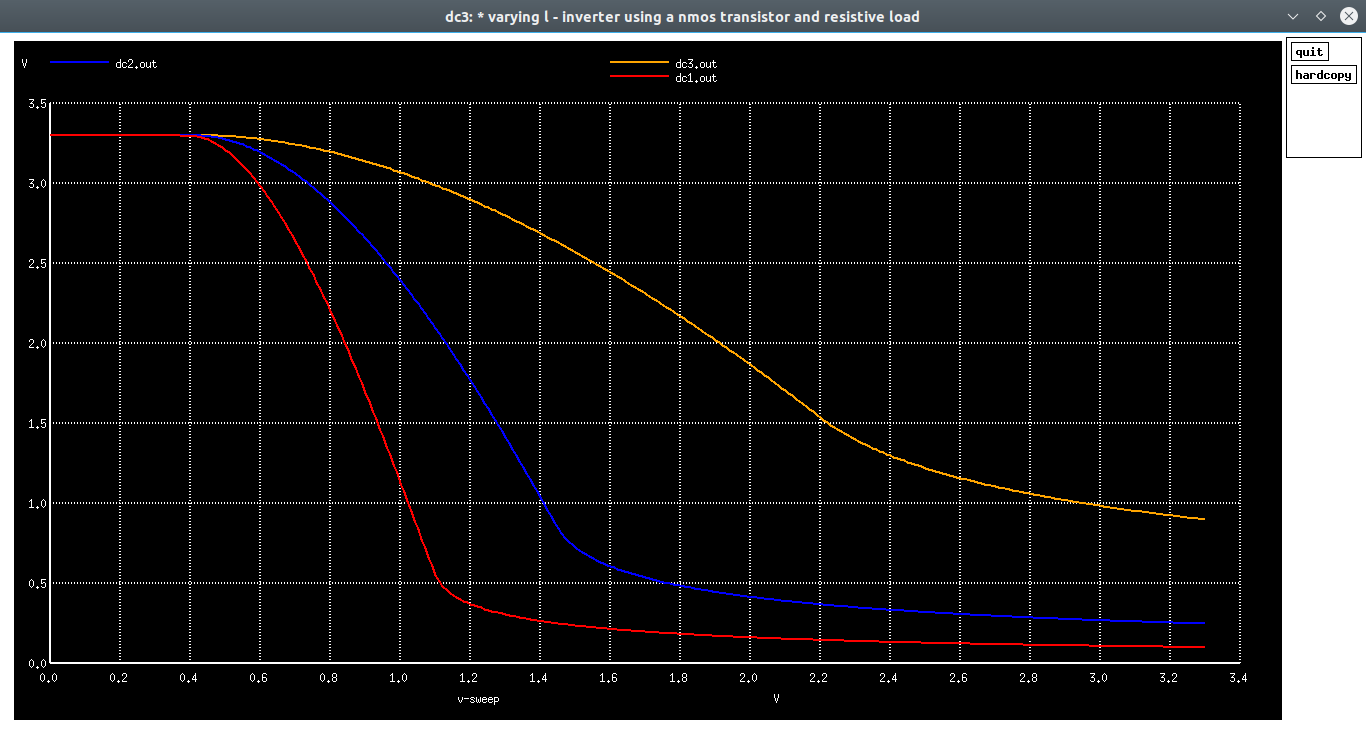
\includegraphics[scale=0.25]{images/inverter_l_dc.png}
			\caption{Transfer Characteristics Varying L}
			\label{fig::varying_l_dc}
		\end{center}
	\end{figure}
	\begin{figure}[H]
		\begin{center}
			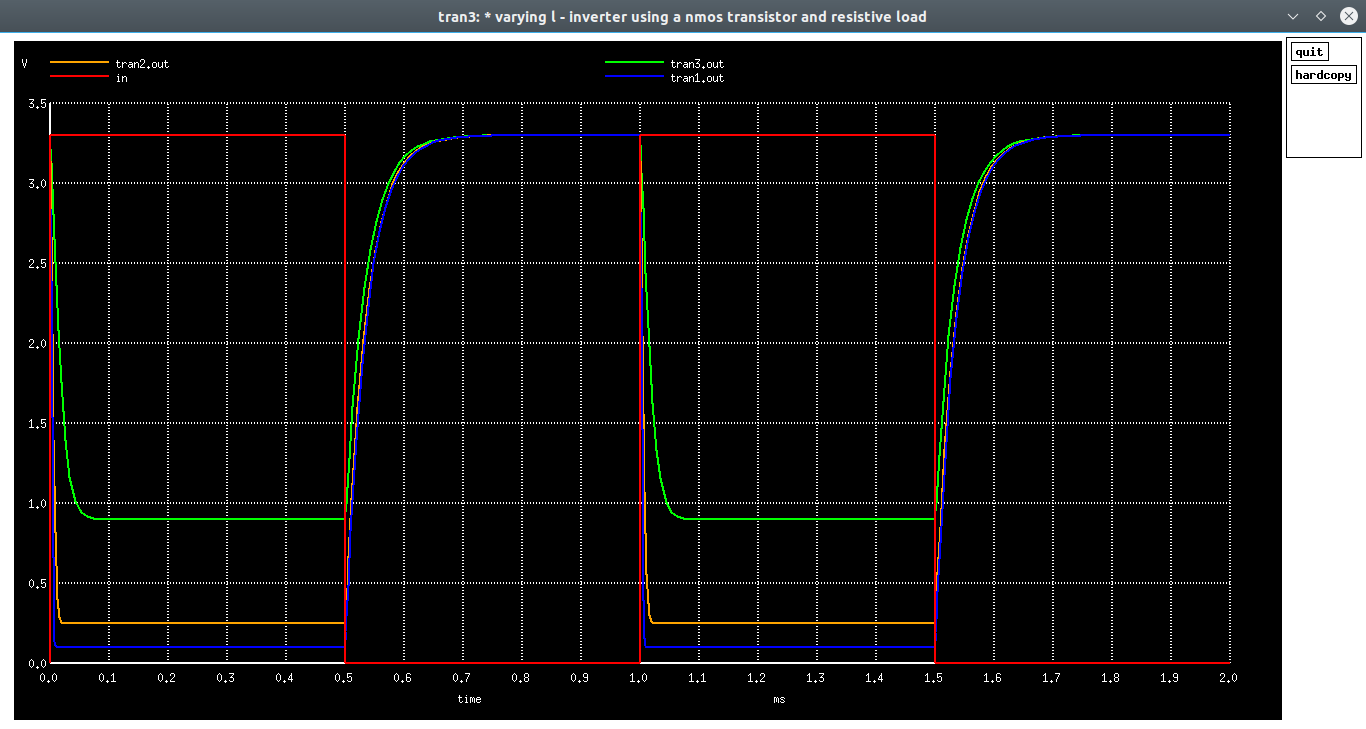
\includegraphics[scale=0.25]{images/inverter_l_tran.png}
			\caption{Transient Response Varying L}
			\label{fig::varying_l_time}
		\end{center}
	\end{figure}
	
	\begin{figure}[H]
		\begin{center}
			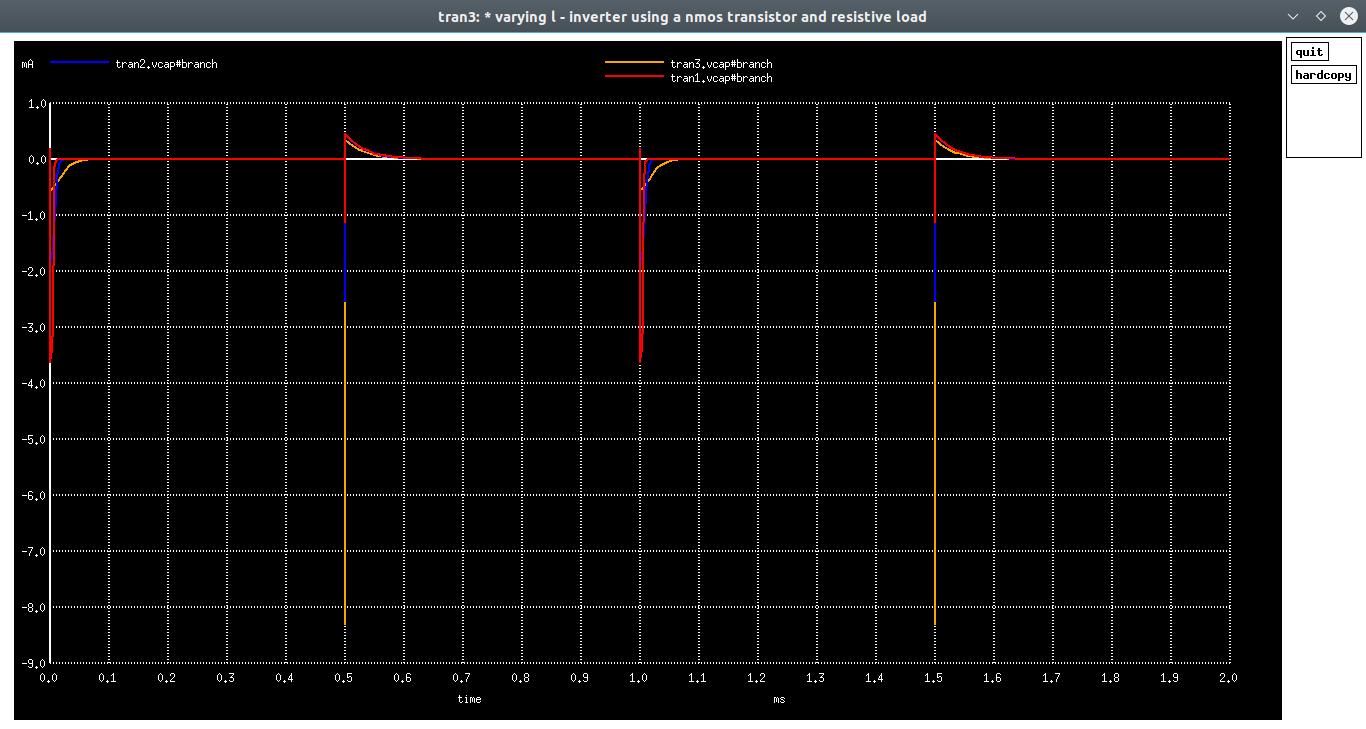
\includegraphics[scale=0.25]{images/inverter_l_vcap.png}
			\caption{Capacitor Current Varying L}
			\label{fig::varying_l_vcap}
		\end{center}
	\end{figure}
	
	\begin{figure}[H]
		\begin{center}
			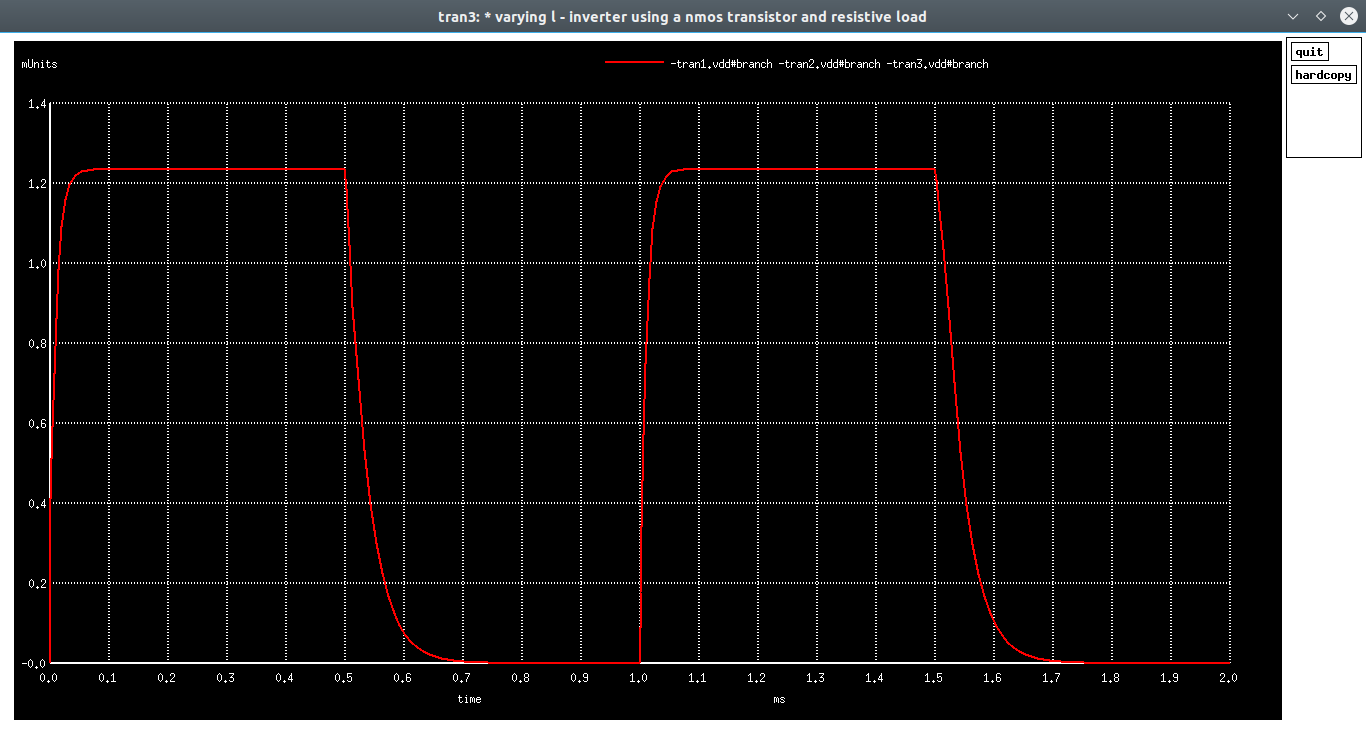
\includegraphics[scale=0.25]{images/inverter_l_vdd.png}
			\caption{Transient Response Varying L}
			\label{fig::varying_l_vdd}
		\end{center}
	\end{figure}
	
    
    
    \newpage
	\section{CMOS Inverter Layout and Characterisation} 
	
	\subsection{Aim}
	
	\subsection{Circuit Diagram}
	\begin{figure}[H]
		\begin{center}
			% XCircuit output "cmos_inverter.tex" for LaTeX input from cmos_inverter.eps
\def\putbox#1#2#3#4{\makebox[0in][l]{\makebox[#1][l]{}\raisebox{\baselineskip}[0in][0in]{\raisebox{#2}[0in][0in]{\scalebox{#3}{#4}}}}}
\def\rightbox#1{\makebox[0in][r]{#1}}
\def\centbox#1{\makebox[0in]{#1}}
\def\topbox#1{\raisebox{-0.60\baselineskip}[0in][0in]{#1}}
\def\midbox#1{\raisebox{-0.20\baselineskip}[0in][0in]{#1}}
   \scalebox{1}{
   \normalsize
   \parbox{1.64583in}{
   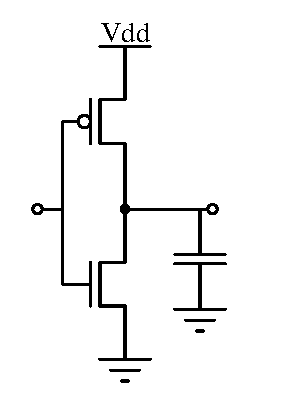
\includegraphics[scale=1]{cmos_inverter}\\
   % translate x=416 y=316 scale 0.38
   \putbox{1.39in}{1.20in}{1.20}{out}%
   \putbox{0.06in}{1.29in}{1.20}{in}%
   \putbox{1.47in}{0.79in}{1.20}{$\text{C}_\text{L}$}%
   } % close 'parbox'
   } % close 'scalebox'
   \vspace{-\baselineskip} % this is not necessary, but looks better

			\caption{Circuit Diagram of CMOS Inverter}
			\label{fig::cmosinvckt}
		\end{center}
	\end{figure}
	
	\subsection{Introduction}
	Inverter is one that inverts the signal supplied at its input. If input is made high or logic level is 1, then the output has a logic level 0 and vice-versa. CMOS stands for Complementary Metal Oxide Semiconductor. CMOS is one of the various families in logic gate design in Digital VLSI. A major difference in this family is, there is both a pull-up network as well as the pull-down network and only one of the path is on at any given time. The output is taken at the junction of pull-up and pull-down network. When pull-up network constructed using PMOS is ON, output capacitor is charged by the supply and when pull-down network constructed using NMOS is ON, the capacitor initially charged now discharges through this path to groun
	
	\subsection{Layout}
	\begin{figure}[H]
		\begin{center}
			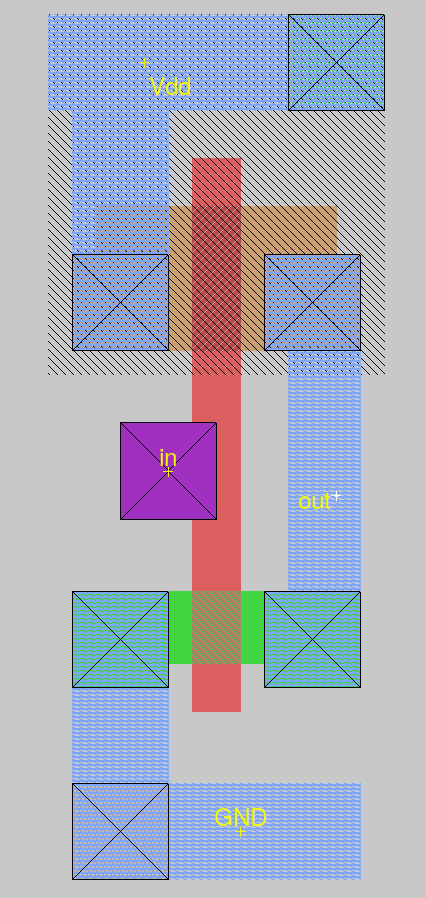
\includegraphics[scale = 0.5]{images/layout.png}
			\caption{Layout of CMOS Inverter}
			\label{fig::cmoslayout}
		\end{center}
	\end{figure}
	
	\subsection{Netlist}
	
	\subsection{Analysis and Observation}
	\begin{figure}[H]
		\begin{center}
			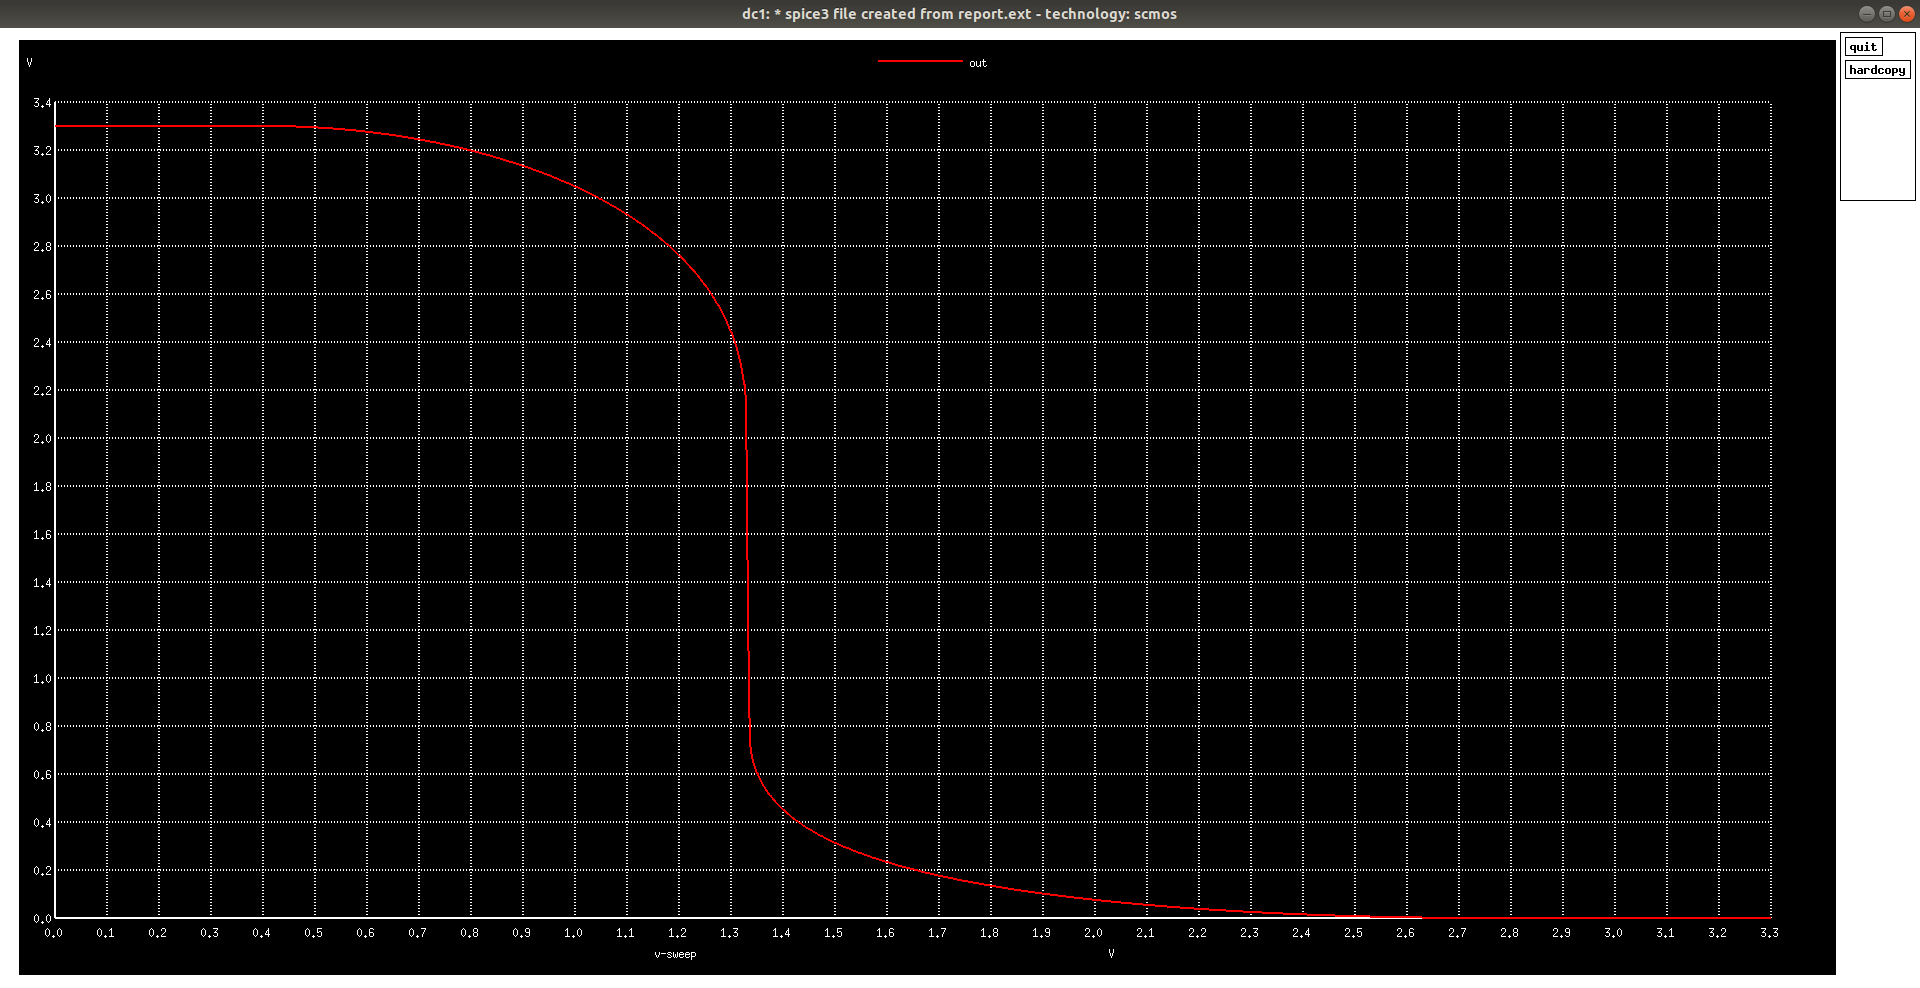
\includegraphics[scale = 0.2]{images/layout_dc.png}
			\caption{CMOS Inverter transfer characteristics}
			\label{fig::layout_dc}
		\end{center}
	\end{figure}
	
	\begin{figure}[H]
		\begin{center}
			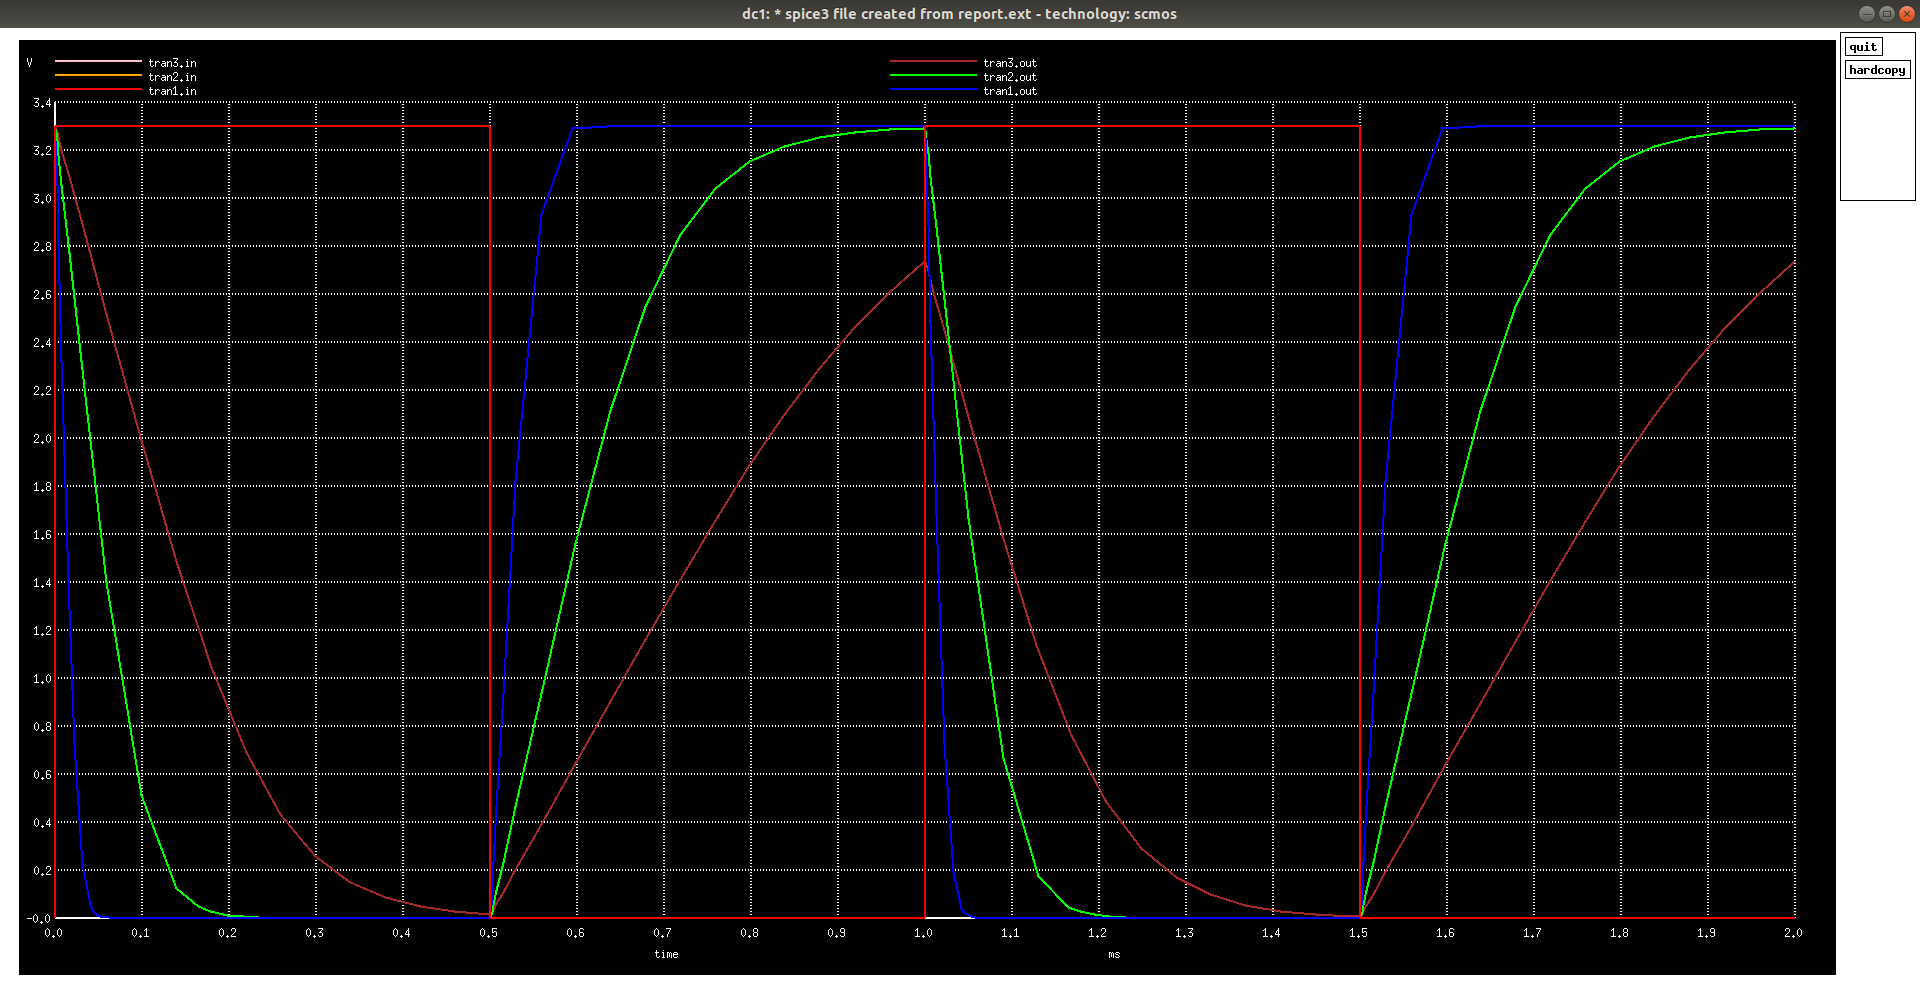
\includegraphics[scale = 0.2]{images/layout_tran_cl.png}
			\caption{CMOS Inverter transient characteristics with various $\text{C}_\text{L}$(5nF, 20nF, 50nF)}
			\label{fig::layout_tran}
		\end{center}
	\end{figure}
	
	
\end{document}